\chapter{The SAFE Network}
\label{ch:thesafenetwork}

\section{Decentralisation}

The decentralisation of data storage is one of the core features that the SAFE Network promises. The internet today is very fragile in that most users don't own or control their own data. When you upload a file to Dropbox\footnote{https://www.dropbox.com} or OneDrive\footnote{https://onedrive.live.com} that file exists solely on the servers that those organisations have control over. Once an organisation has data they can do with it what they wish, acting within the bounds of overcomplicated privacy polices to manage user data. Not only can this incur privacy infringements but it can lead someone into the false sense of security that their data is safe. If someone managed to hack Dropbox or there was a catastrophic failure at the datacenter, a user has no assurances that their data is safe. On a much larger scale companies like Amazon provide AWS\footnote{https://aws.amazon.com/}, an enterprise grade cloud-computing platform. If AWS were to fail, or be the target of a hack, many of the worlds biggest websites would cease to function. This is because of the centralisation of resources. Services like AWS are not easy to target, but they are a single and identifiable part of the equation. A chain is only as strong as its weakest link. 

Trust is at the core of decentralisation. Centralised control of resources requires trust in the facilitators of that resource. You have to trust that the resource is free of corruption and indeed trust that it won't be in the future. Companies readily change polices upon acquisition and managerial changes so this trust has to withhold over the course of time. Decentralised models of governance can be used to alleviate these problems. Through autonomous governance, entities such as the SAFE Network can ensure equality to all participants. It achieves this through a system of ``trust-less'' cooperation, \textit{vaults} on the network do not inherently trust other \textit{vaults}. Every action on the network must reach a quorum before it is considered valid by the \textit{vaults}. This autonomous self-governance is what decentralises the ``trust'' you must impart on the network.

\subsection{Peer to Peer vs Client Server}

Centralisation of data and computing power is a natural consequence of the client-server architecture that has formed around the internet. It requires trust in the server you are interacting with. When a user want to upload data that trust in the entity becomes a big consideration. The client-server architecture forces centralised governance and inequality between the participants in the network. A Peer to Peer (P2P) network encourages the decentralisation of power. In a P2P network, participants are often of equal standing meaning no node in the network has more authority than any other node. Thus for a true decentralised network you have to have a P2P architecture to support it.

The SAFE Network thus has to be built around the P2P architectural model. Nodes that comprise the SAFE Network are called \textit{vaults}. \textit{Vaults} are responsible for both storing and serving data, they work together through an autonomous system of governance. Some \textit{vaults} in the network do have more authority than others, these \textit{vaults} are called \textit{elders}. To become an \textit{elder} a \textit{vault} must first prove it is trustworthy and only after a quorum is reached between other vaults can it become an \textit{elder}. A \textit{vault} of this status has more voting power than other vaults, using this power to reach agreements with other \textit{elders} and \textit{vaults} on all network decisions. This decentralised self-governance scheme is crucial to the autonomy and reliability of the network.

\begin{figure}
	\begin{center}
		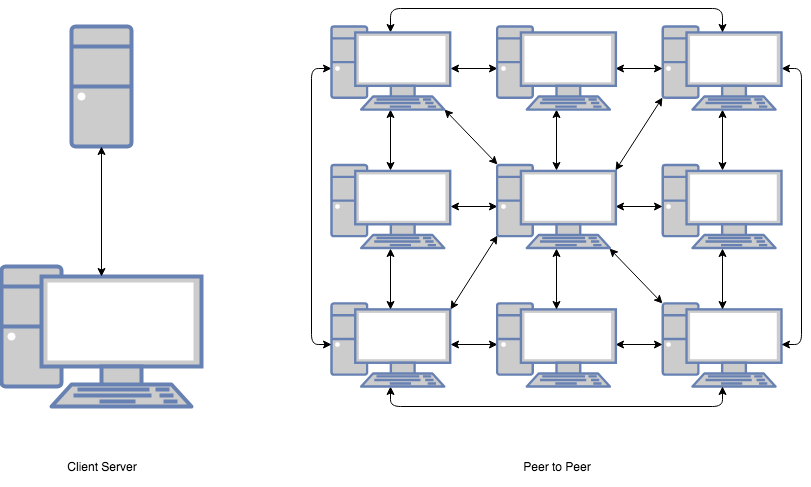
\includegraphics[width=\textwidth]{diagrams/client-server-vs-p2p}
		\caption{Client-Server vs Peer-to-Peer Network}
		\label{fig:client-server-peer2peer}
	\end{center}
\end{figure}

\subsection{BitTorrent}

The first stable version of the BitTorrent\cite{cohen2008bittorrent} protocol was released in 2001. Since then it has become one of the worlds most popular means of file sharing, accounting for \%3.5 of global internet traffic at the time of writing\cite{bittorrent-usage}. In a \textit{permission-less} environment users are allowed to freely share files with one another. As there is no centralised body controlling who has access to what data, the system has been widely used for the piracy of copyrighted material. The SAFE Network aims to solve many of the same problems that BitTorrent does. One of which is moving away from the traditional client-server architecture of file sharing. In BitTorrent, \textit{peers} form what is known as a \textit{swarm}. A \textit{swarm} is all nodes that aim to download a full copy of a piece of data. Data is broken down into discrete chunks, each with a unique hash that allows nodes to uniquely identify each piece of the original file. A node in the \textit{swarm} is known as a \textit{peer} when they don't hold a complete copy of the file. A node in the \textit{swarm} is referred to as a \textit{seed} when they do hold a complete copy of the file. The ``resting state'' of this network is when all nodes in the \textit{swarm} are \textit{seeds}. Nodes in the \textit{swarm} offer the file chunks that they have to other nodes and then use P2P routing to send the file chunks between one another.

In BitTorrent there is no central server to attack (disregarding a \textit{tracker}, there are \textit{tracker-less} solutions available). The topology of a \textit{tracker} based \textit{swarm} can be seen in Figure \ref{fig:bittorrent-tracker}. Nodes can leave and rejoin the \textit{swarm} whenever they want, as long as at least one node has a copy of a specific chunk then all nodes in the \textit{swarm} can spread the data and become \textit{seeders}. This level of data redundancy is a huge benefit to BitTorrent over a traditional client-server model of sharing files.

\begin{figure}
	\begin{center}
		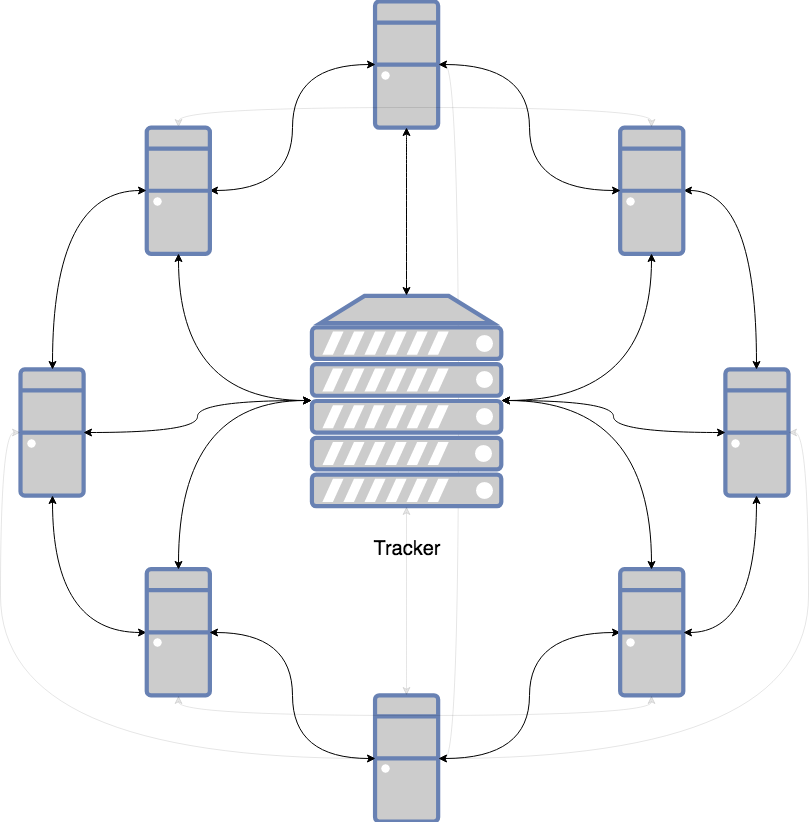
\includegraphics[scale=0.3]{diagrams/bittorrent}
		\caption{Topology of tracker based swarm in BitTorrent}
		\label{fig:bittorrent-tracker}
	\end{center}
\end{figure}

In the client-server model of file sharing, the owner of the server incurs great cost in the hosting of the file. They have to pay for the management, storage and network costs that are associated with serving that data. For large companies this is often a negligible cost that is not a prohibiting factor in hosting the data. For smaller organisations however (especially non-profits) this server cost can be a big problem. This is a primary reason why many Linux distributions so often provide BitTorrent links to download the operating system. By using BitTorrent they can offload the cost of file sharing onto their users. This works on a ``good-samaritan'' basis where a node should aim to serve as much data as they themselves have received from the \textit{swarm}. For the vast majority of users this cost is negligible and can act as a ``good-will'' gesture to help support projects.

Data transfer speeds are a major benefit of using BitTorrent and other P2P file sharing methods. When a node is acting as a \textit{peer}, their download speed is limited to the summation of the upload speeds of the nodes they are connected to. This often means that in a well established \textit{swarm}, download speed is only limited by the nodes internet connection. The more nodes that join the \textit{swarm}, the faster and more resilient to failures the network gets. This is juxtaposed to a client-server model wherein a single connection to the server must be shared by all the nodes wishing to download the data. Thus download speeds are limited by the resources of that single server.

BitTorrent may solve many issues surrounding the distribution of files, but falls short of solving the decentralisation of the internet as a whole. The main limitation being that data on BitTorrent is not mutable. Once a file has been spread to a \textit{swarm} it is an immutable entity that cannot be changed. This means it is extremely challenging to use BitTorrent for dynamic content such as websites. Immutability is a big drawback depending on the use case, thus the option to support both Mutable and Immutable data is beneficial. The other attributing factor is that data only exists inside \textit{swarms}, a node cannot interact with data without first joining the relevant \textit{swarm}. So the discoverability of data is also an issue. These are all points that the SAFE Network offers solutions to.

\section{Serverless Architecture}

The idea behind a serverless architecture is to move as much computation and functionality to the client as possible. As time passes, the computational power of user workstations gets faster. This computational power goes wasted for the most part. While browsing the internet, interacting with Facebook for instance, a computer actually does very little in terms of processing the information a user sees. Facebook serves to the browser a thin-client which can then make requests to Facebook for the data that is needed. Thus there is untapped potential on the client to perform more work locally instead of doing it on a server. 

There are drawbacks in offloading work to the client. The first issue, especially with websites like Facebook, is privacy. When Facebook processes data on their servers, they can assure that only data a user is allowed to see is sent to the client. If all data had to be processed locally it would introduce new challenges in data protection and security. Another drawback is that of mobile devices. On laptops, smartphones, tablets and IoT devices, power consumption is a major problem. Thus by using the client-sever model, electricity expensive computation can be offloaded to the server and reduce power consumption on the client. This is in combination with reducing network traffic to the client, which for mobile devices is a crucial factor in battery life. Thus computation and power consumption on mobile devices means that client-server makes more sense than the serverless architectural model.

\textit{Vaults} serve a similar purpose to \textit{peers} in BitTorrent. Note that they do not serve a similar function to \textit{seeds}, the SAFE Network aims to never keep a complete copy of a single file stored on one \textit{vault}. The SAFE Network in this capacity can then facilitate file sharing just like BitTorrent. Additionally what the SAFE Network has is the ability to route requests throughout the entire network. All \textit{vaults} in the network have the knowledge required to find any chunk of data. This is different to a node in BitTorrent because it can only find a chunk of data within the \textit{swarms} it knows about. As this dynamic routing exists, the SAFE Network has a form of DNS that can be used. Another major difference is that the SAFE Network is capable of mutable data. This means that the SAFE Network is fully capable of supporting dynamic websites, forums, email and other such applications. A user can open a browser that is capable of connectivity with the SAFE Network and browse the \textit{internet} just as they would normally.

\textit{Vaults} cannot process data thus SAFE Network applications must process data locally and only use the network as a storage and transport medium. Thus the serverless architectural model is a good fit for the SAFE Network. This style of building websites and applications has been around for a long time. With the advent of JavaScript and other such technologies, it was possible to run code locally through the browser without needing the server to do any processing. A good example is online mini-games, the code runs locally and there is no processing required on the server. The JavaScript/Flash/Java/... is served to the client and the processing is performed locally. Another example of this are online ``office suites'', they are very powerful programs that can be ran through the browser. They depend heavily on the processing power of the client to provide an experience similar to that of a desktop application.

Unless the SAFE Network is just used as a component in the stack, it forces the serverless architecture model to be used. This introduces challenges in how applications are designed and built. As development is entirely focused on the client, development time on the back-end can be eliminated. Instead of designing websites and applications the \textit{traditional} way, they must be developed as fat-clients. Websites will become heavier, requiring more care and optimisations. Messy and slow JavaScript is common on the internet today, mostly due to the abundance of computing power that exists. As discussed previously, battery life is an important consideration when offloading work to the client. This means that applications/websites that follow the serverless architectural model must be well optimised for power consumption. A new technology called Web Assembly is gaining traction and could help alleviate these issues.

\subsection{Web Assembly}

Web Assembly is an assembly-like language that can be compiled to from C, C++, Rust, etc, and then ran inside web browsers. It allows code to be written in high-level languages (that aren't interpreted like JavaScript) and then ran on the client with \textit{near native} performance. This has big implications for the internet as a whole, not just the SAFE Network. A technology like Web Assembly could therefore be extremely useful when building websites that use the serverless architectural model. A big strength of Web Assembly is in the processing of data. Optimised and high performance code to process data can be more easily written in languages like C than in languages like JavaScript. Since the SAFE Network serves raw data to the client, the use of Web Assembly to process that data could be of huge benefit.

\subsection{Serverless Fat Clients}

Although not all fat-clients follow the serverless architectural model, applications that are designed to be serverless are inherently fat-clients. Hence because of the points mentioned previously, the SAFE Network encourages (almost requires) the fat-client style of architecture to be used for software development. As web technologies mature they become more suitable for the development of fat-clients. Instead of having to download desktop applications to a device, new technologies allow powerful applications to be built and delivered through the web. If delivering fat-client applications through the web was not possible, users would have to download apps for popular services like YouTube, Facebook, Twitter, etc. Hence the advent of new web technologies, such as Web Assembly, is an enabler in the success of the SAFE Network.

\section{Ownership of Data}
\label{sec:ownership-of-data}

Accessing the SAFE Network is \textit{permission-less}. What this means is that users don't need to go to a central body that controls the network to ask for (register) an account. A user simply connects to the network and is allowed to create one. All users of the network are equal, there is no concept of ``admin'' accounts. When a user uploads a piece of data to the network, it can either be ``public'' data or encrypted data. Note that all data stored by \textit{vaults} is encrypted, if the data is ``public'' then it simply means that the decryption key is publicly derivable so anyone can access the data.

Ownership of data is one feature that the SAFE network provides as apposed to a system like BitTorrent. All nodes in BitTorrent have equal rights to data, so a node can't simply delete or edit a file once it has been spread to the \textit{swarm}. In the SAFE Network, the ownership of data is more clearly defined. When data is uploaded it is split into chunks and distributed across different \textit{vaults}. That data has an identifiable ``owner'', the account that originally uploaded it to the network and has the relevant decryption keys. A special type of data called Mutable Data can be edited and controlled by its ``owner'' while still being stored and managed by the network. The ``owner'' maintains ``control'' over that data.

In the SAFE Network users ``own'' and control their own data, nobody else can edit or tamper with it. This does however incur issues surrounding the distribution of illicit and copyrighted content. One could imagine a user uploading the latest Hollywood blockbuster and sharing the link to it. As data cannot be deleted that file will be available forever. A solution to this could be through the use of a \textit{master-key} to the network. This would be a key that would allow complete access to the network and unlock the ability to delete data. Such a key would be beneficial in removing illicit content but completely invalidates the principles of the SAFE Network. This issue of control has made a huge impact upon BitTorrent. Numerous court cases and law suits have been issued since its inception due to its use for illicit content distribution. This is a situation of ``you can't have your cake and eat it to''. It is impossible to ensure complete security of user data and then undermine that with the ability of a central body to tamper with it. Like BitTorrent the SAFE Network is a tool. Users will do with it what they wish. The mitigation against those who wish to use a tool for illegal activities should not impact upon those who follow the law.

\section{Architecture of the SAFE Network}

The SAFE Network is still in active development. At the time of writing, the SAFE Network is currently on its second alpha revision (Alpha 2) out of a planned four. Thus the architecture of the SAFE Network is still subject to rapid change. Chapter \ref{ch:architecture} explains the architecture of the SAFE Network at the time of writing.